\subsection{Set}

In questo capitolo ci troviamo ad affrontare l'implementazione dei \textit{\textbf{set,}} la loro struttura rimarca la struttura dati matematica degli insiemi e con essa anche le operazioni annesse.

Come già consetudine anche in questo capitolo affronteremo la parte teorica, esploreremo i vari casi d'uso correlati di esempi pratici.

\subsection{Caretteristiche Fondamentali}\label{fondamentsSet}
Come già accennato ad inizio capitolo i \textit{\textbf{set}} si rifanno alla teoria degli insiemi matematici, quindi prima di esplorare i \textit{\textbf{set}} in Python è bene conoscere la teoria degli insiemi.

\subsubsection{Teoria degli insiemi}\label{TeoriadegliInsiemi}

In matematica un insieme rappresenta una collezione di oggetti, \textit{non ordinati, distinti}, ogni oggetto, (in matematichese denominato elemento) può appartenere o non all'insieme, senza possibilità di duplicazione o ordinamento intrinseco.

Una definizione formale stabilisce che due insiemi sono uguali se e solo se contengono esattamente gli stessi elementi, indipendentemente dall'ordine in cui questi sono disposti, stessa considerazione avviene in Python, dove l'identità della collezione dipende esclusivamente dal contenuto e non dalla sequenza di disposizione.

\subsubsection{Uguaglianza e Principio di Estensionalità}\label{EstensionalitàSet}

Il principio di estensionalità stabilisce che due insiemi sono uguali se e solo se contengono esattamente gli stessi elementi. Questo principio implica che l'ordine di enumerazione degli elementi è irrilevante per determinare l'identità dell'insieme, così come il numero di volte in cui un elemento viene menzionato. 


Gli insiemi {1, 2, 3}, {3, 1, 2}, e {1, 2, 3, 1} rappresentano la medesima entità matematica.
Questa proprietà fondamentale si traduce direttamente nel comportamento dei set Python, dove l'operatore di uguaglianza verifica la coincidenza degli elementi indipendentemente dall'ordine di inserimento o dalla presenza di tentativi di inserimento duplicati.


\subsubsection{Operazioni tra Insiemi}\label{OperazioniTraInsiemi}

Iniziamo ad affrontare le operazioni possibili tra insiemi, dato che sono equivalenti con le operazioni tra \textit{\textbf{set}} in Python.

\paragraph{Unione tra Insiemi}
L'unione di due insiemi A e B in matematica equivale all'insieme contenente tutti gli elementi che appartengono ad \textbf{A} e a \textbf{B}


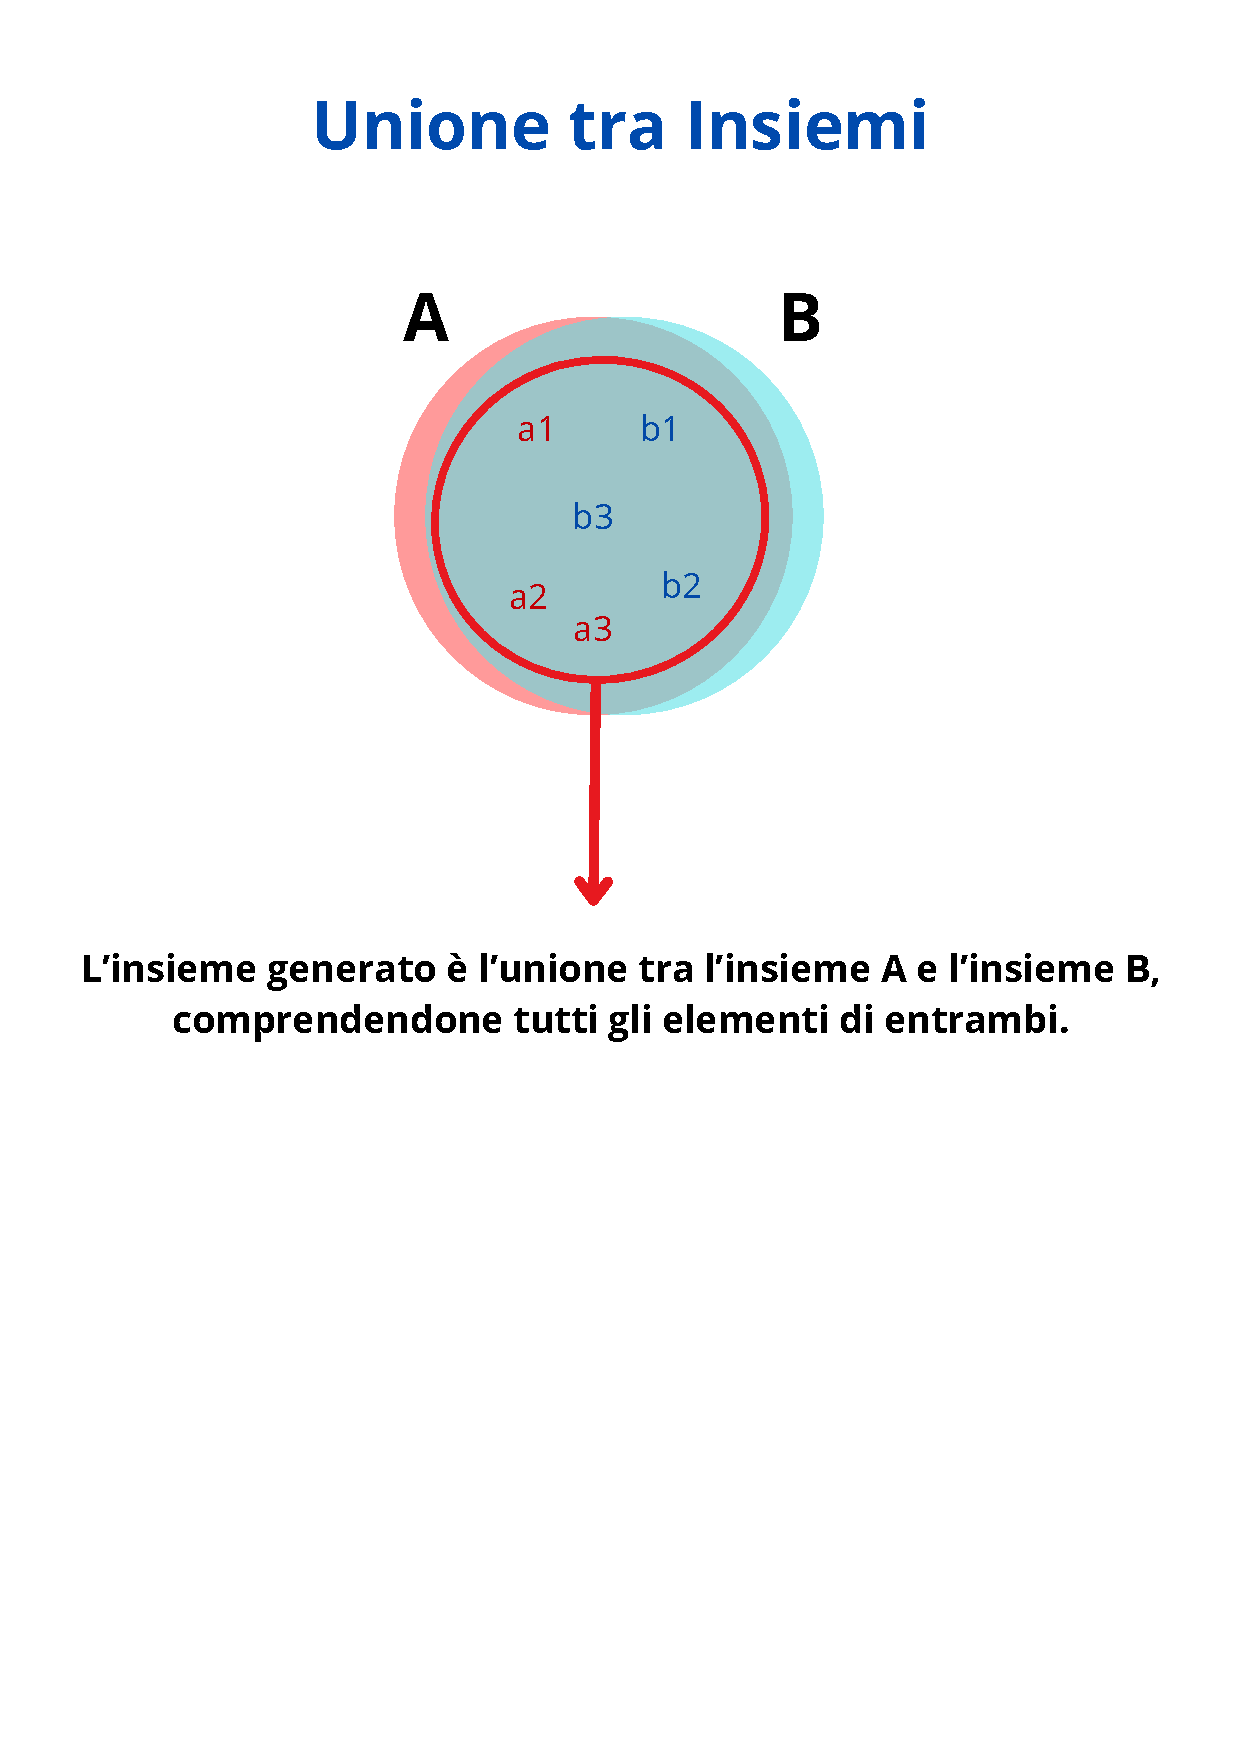
\includepdf[pages=-,scale=0.75,pagecommand={\thispagestyle{empty}},fitpaper=true]{pdf/Unione Insiemi.pdf}

\paragraph{Intersezione tra Insiemi}
L'intersezione tra insiemi, invece, comprende solo gli elementi comuni tra gli insiemi.

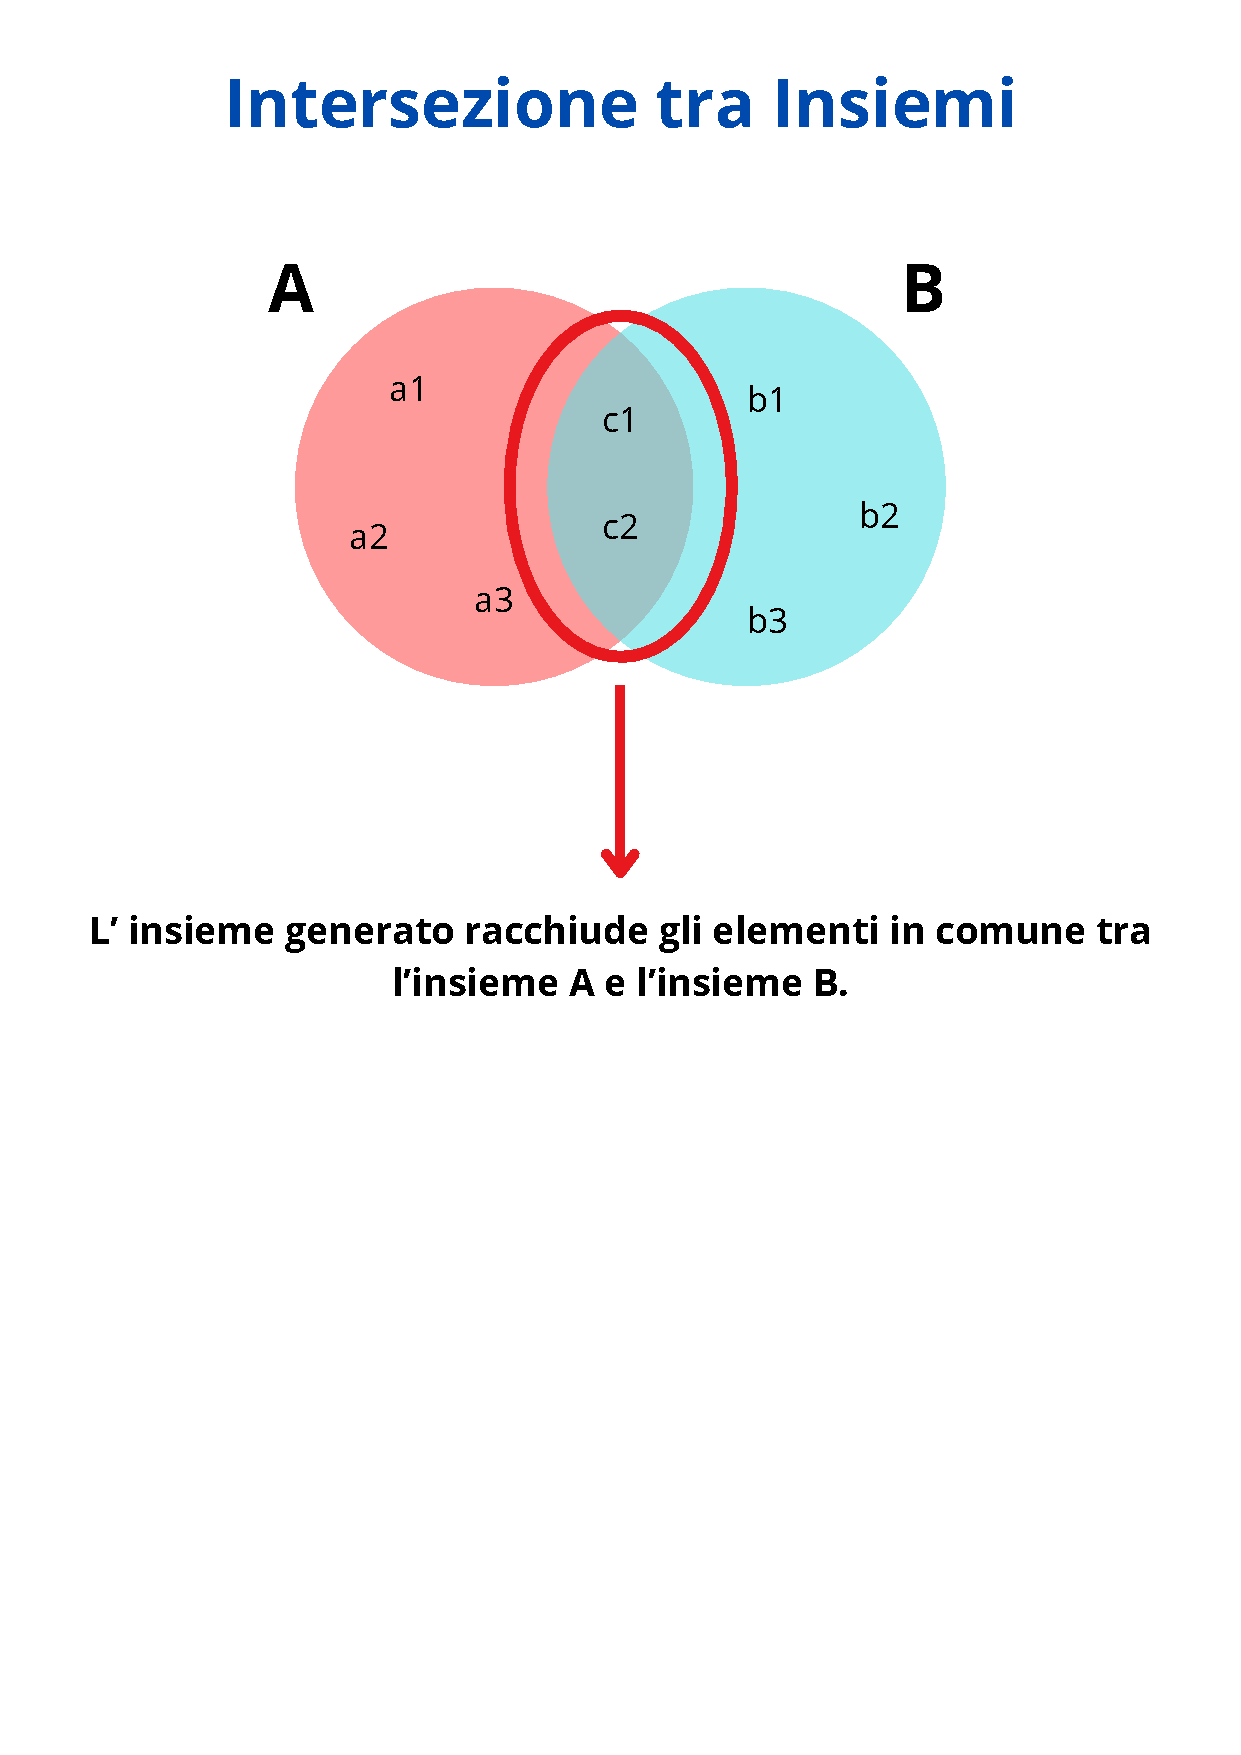
\includepdf[pages=-,scale=0.75,pagecommand={\thispagestyle{empty}},fitpaper=true]{pdf/Intetrsezione insiemi.pdf}


\paragraph{Differenza tra Insiemi}

L'operazione di differenza tra insiemi, A - B, non è altro che l'insieme contenente tutti gli elementi che appartengono ad A ma non a B



Un'altra operazione in comune tra i \textit{\textbf{set}} e gli insiemi matematici è quella della differenza simmetrica tra insiemi, come è facile intuire dal nome dell'operazione, l'insieme risultante sarà dato soltanto dagli elementi non comuni tra gli insiemi esaminati.